%%%%%%%%%%%%%%%%%%%%%%%%%%%%%%%%%%%%%%%%%
% University Assignment Title Page 
% LaTeX Template
% Version 2.1 (18/10/18)
% Modified by
% Erdem TUNA &
% Halil TEMURTAŞ &
% Enes TAŞTAN
%%%%%%%%%%%%%%%%%%%%%%%%%%%%%%%%%%%%%%%%%
%
%----------------------------------------------------------------------------------------
%	PACKAGES AND OTHER DOCUMENT CONFIGURATIONS
%----------------------------------------------------------------------------------------
\documentclass[a4paper,12pt]{article}
%-----packages------
\usepackage[a4paper, total={6.2in, 9in}]{geometry}
\usepackage[english]{babel}
\usepackage[utf8x]{inputenc}
\usepackage{amsmath}
\usepackage{graphicx}
\usepackage[colorinlistoftodos]{todonotes}
\usepackage{gensymb} % this could be problem
\usepackage{float}
\usepackage{fancyref}
\usepackage{subcaption}
\usepackage[titletoc]{appendix} %appendix package
\usepackage{xcolor}
\usepackage{listings}
\usepackage{xspace}
\usepackage{amssymb}
\usepackage{nicefrac}
\usepackage{gensymb}
\usepackage{fancyhdr}
\usepackage{lipsum}  % for dummy text \lipsum[1-4]
\usepackage[final]{pdfpages}  % pdf include
%\usepackage{array} %allows more options in tables
\usepackage{pgfplots,pgf,tikz} %coding plots in latex
%\usepackage{capt-of} % allows caption outside the figure environment
\usepackage[export]{adjustbox} %more options for adjusting the images
%\usepackage{multicol,multirow,slashbox} % allows tables like table1
%\usepackage[hyperfootnotes=false]{hyperref} % clickable references
%\usepackage{epstopdf} % useful when matlab is involved
%\usepackage{placeins} % prevents the text after figure to go above figure with \FloatBarrier 
%\usepackage{listingsutf8,mcode} %import .m or any other code file mcode is for matlab highlighting
\usepackage{setspace}
%-----end of packages




%-----specifications-----
\definecolor{mGreen}{rgb}{0,0.6,0} % for python
\definecolor{mGray}{rgb}{0.5,0.5,0.5}
\definecolor{mPurple}{rgb}{0.58,0,0.82}
\definecolor{mygreen}{RGB}{28,172,0} % color values Red, Green, Blue for matlab
\definecolor{mylilas}{RGB}{170,55,241}

\setcounter{secnumdepth}{5} % how many sectioning levels to assign numbers to
\setcounter{tocdepth}{5}    % how many sectioning levels to show in ToC

\lstdefinestyle{CStyle}{
	commentstyle=\color{mGreen},
	keywordstyle=\color{magenta},
	numberstyle=\tiny\color{mGray},
	stringstyle=\color{mPurple},
	basicstyle=\footnotesize,
	breakatwhitespace=false,         
	breaklines=true,
	frame=single,
	rulecolor=\color{black!40},                 
	captionpos=b,                    
	keepspaces=true,                 
	numbers=left,                    
	numbersep=5pt,                  
	showspaces=false,                
	showstringspaces=false,
	showtabs=false,                  
	tabsize=2,
	language=C
}

\lstset{language=Matlab,%
	%basicstyle=\color{red},
	breaklines=true,%
	frame=single,
	rulecolor=\color{black!40},
	morekeywords={matlab2tikz},
	keywordstyle=\color{blue},%
	morekeywords=[2]{1}, keywordstyle=[2]{\color{black}},
	identifierstyle=\color{black},%
	stringstyle=\color{mylilas},
	commentstyle=\color{mygreen},%
	showstringspaces=false,%without this there will be a symbol in the places where there is a space
	numbers=left,%
	numberstyle={\tiny \color{black}},% size of the numbers
	numbersep=9pt, % this defines how far the numbers are from the text
	emph=[1]{for,end,break},emphstyle=[1]\color{red}, %some words to emphasise
	%emph=[2]{word1,word2}, emphstyle=[2]{style},    
}


\tikzset{
	desicion/.style={
		diamond,
		draw,
		text width=4em,
		text badly centered,
		inner sep=0pt
	},
	block/.style={
		rectangle,
		draw,
		text width=10em,
		text centered,
		rounded corners
	},
	cloud/.style={
		draw,
		ellipse,
		minimum height=2em
	},
	descr/.style={
		fill=white,
		inner sep=2.5pt
	},
	connector/.style={
		-latex,
		font=\scriptsize
	},
	rectangle connector/.style={
		connector,
		to path={(\tikztostart) -- ++(#1,0pt) \tikztonodes |- (\tikztotarget) },
		pos=0.5
	},
	rectangle connector/.default=-2cm,
	straight connector/.style={
		connector,
		to path=--(\tikztotarget) \tikztonodes
	}
}

\tikzset{
	desicion/.style={
		diamond,
		draw,
		text width=4em,
		text badly centered,
		inner sep=0pt
	},
	block/.style={
		rectangle,
		draw,
		text width=10em,
		text centered,
		rounded corners
	},
	cloud/.style={
		draw,
		ellipse,
		minimum height=2em
	},
	descr/.style={
		fill=white,
		inner sep=2.5pt
	},
	connector/.style={
		-latex,
		font=\scriptsize
	},
	rectangle connector/.style={
		connector,
		to path={(\tikztostart) -- ++(#1,0pt) \tikztonodes |- (\tikztotarget) },
		pos=0.5
	},
	rectangle connector/.default=-2cm,
	straight connector/.style={
		connector,
		to path=--(\tikztotarget) \tikztonodes
	}
}
%-----end of specifications-----


%----commands----
\newcommand\nd{\textsuperscript{nd}\xspace}
\newcommand\rd{\textsuperscript{rd}\xspace}
\newcommand\nth{\textsuperscript{th}\xspace} %\th is taken already
\newcommand{\specialcell}[2][c]{ \begin{tabular}[#1]{@{}c@{}}#2\end{tabular}} % for too long table lines

\newcommand{\blankpage}{
	\- \\[9cm]	
	{ \centering \textit{This page intentionally left blank.} \par }
	\- \\[9cm]
}% For Blank Page

\makeatletter
\renewcommand\paragraph{\@startsection{paragraph}{4}{\z@}%
	{-2.5ex\@plus -1ex \@minus -.25ex}%
	{1.25ex \@plus .25ex}%
	{\normalfont\normalsize\bfseries}}
\makeatother
%-----end of commands-----
\onehalfspacing
\begin{document}

\begin{titlepage}

\newcommand{\HRule}{\rule{\linewidth}{0.5mm}} % Defines a new command for the horizontal lines, change thickness here
\centering 


\includegraphics[width=\textwidth,height=\textheight,keepaspectratio]{../../Documents/logos/logo3-with-stroke}\\[0.5cm]

\textsc{\LARGE Middle East Technical University}\\[0.5cm] % Name of your university/college
\textsc{\Large Department of \\Electrical and Electronics Engineering }\\[0.5cm] % Major heading such as course name
\textsc{\large EE493 ENGINEERING DESIGN I}\\[0.5cm] % Minor heading such as course title


\HRule \\[0cm]
{ \huge \bfseries  Car Chasing Robot\\[0.1cm] \LARGE \bfseries Proposal Report}\\[0cm] % Title of your document
\HRule \\[1cm]

\begin{minipage}[l]{0.6\textwidth}
\raggedright
		\large{\textbf{Supervisor:}}	Assoc. Prof. Emre Özkan \\
		\hspace{3.05cm}\color{red}  METU EE / C-206

\end{minipage}
\begin{minipage}[r]{0.35\textwidth}
\raggedright
		\textbf{Project Start:} 4/10/2018\\
		\textbf{Project End:} \ \  26/5/2019\\
		\textbf{Project Budget:} \$450

\end{minipage}\\[1cm]
\begin{minipage}{\textwidth}
	\begin{flushleft}
		\large{\textbf{Company Name :}}	Duayenler Ltd. Şti.\\
		\begin{table}[H]
			\begin{tabular}{l l l l}
				\hline
				\textbf{Members}&\textbf{Title}& \textbf{ID}&\textbf{Phone} \\ \hline
				Sarper Sertel & Electronics Engineer& 2094449 & 0542 515 6039  \\ 
				Enes Taştan & Hardware Design Engineer & 2068989 & 0543 683 4336  \\ 
				Erdem Tuna & Embedded Systems Engineer& 2617419 & 0535 256 3320  \\ 
				Halil Temurtaş & Control Engineer& 2094522 & 0531 632 2194  \\
				İlker Sağlık & Software Engineer& 2094423 & 0541 722 9573  \\ \hline
				
				
			\end{tabular}
		\end{table}
	\end{flushleft}
\end{minipage}\\[1cm]

\begin{flushbottom}
{\large November 9, 2018} % Date, change the \today to a set date if you want to be precise
\end{flushbottom}

\end{titlepage}

\blankpage
\tableofcontents
\newpage



\section{Executive Summary}

	Increasing demand on automobiles, encourages industry to produce more. The increase of car count in the traffic, makes the traffic flow more complex. In this scope, autonomous cars bring an innovative solution for reducing the complexity. Potential benefits of automated cars include smart use of fuel, safer traffic and increased mobility. To realize and come up with such solutions, DUAYENLER Ltd. Şti. (DUAYENLER) is founded by five innovative and enthusiast electronics engineering students to intelligently automate the future of traffic.\\
	
	DUAYENLER is composed of talented and diligent people from different disciplines to complete the envisioned problem. DUAYENLER consists of two engineers from computer area, two from electronics area and one from control area. Since realization of the problem requires combinations of different disciplines, DUAYENLER is qualified to accomplish the encountered problems.\\
	
	DUAYENLER will address the need of autonomous cars. Thus, the aim of the proposed project is to design and construct a vehicle that can follow a closed path without a driver on board. Furthermore, the vehicle will be able to sense other vehicles on the road as well as handling the obstacles.\\
	
	The vehicle will use camera vision and sensors to detect and understand environment. With the obtained data, the vehicle will operate in a way that it adjusts its direction and speed correctly. Additionally, if the vehicle detects another vehicle within 5 cm either at the front or at the back, it will activate the handshake protocol to communicate with the opponent and stop with positive signal.\\
	
	The duration of the project is intended to last 33 weeks, starting from October, 1 2019 and ending in May, 26 2019. The estimated cost for research and development phase is  \$ 450 whereas mass production cost per vehicle will be at most \$ 200. Along with the vehicle itself, DUAYENLER will provide its customers with deliverables such as user and technical manuals, elliptical race path, chargeable battery and battery charger. Also, the vehicle will have two (2) years of warranty.
	

\section{Introduction}

	Driving is a common event that many people experience in their daily life. As time passes, human reflexes started to become insufficient for driving compared to fast pace of daily life in modern world. Together with the developments in the technology, new solutions are proposed to assist the driver such as lane tracking and emergency breaking systems. The ultimate version of such solutions are considered to be fully autonomous self-driving cars. \\

Self-driving vehicles are presented to the society as a solution that can facilitate people's life in many ways. Fast operation of the electronics system allows faster response than humans can. A fast and reliable operation of self-driving action can prevent many accidents and increase the safety of the roads in heavy traffics since the system is immune to human defects such as distraction and panic. As a result, autonomous vehicles can open doors to a safer and more conventional future.\\

DUAYENLER Ltd. Şti. is launched with the aim of innovating automation technologies. In that context, a device that can detect the road and other vehicles on them will be built. It autonomously track the lane and stay on the road while trying to as fast as possible.\\

This report includes;
\begin{itemize}
	\item Organization of the company by explaining of the qualifications of the members. 
	\item Requirements for physically realizing the intended vehicle
	\item Possible solutions in system and subsystem levels by explaining their operations
	\item Timeline and cost of the project
	\item Expected deliverables from the project 
\end{itemize} 



\section{The Team}

	DUAYENLER Ltd. Şti. (DUAYENLER) was founded in September 2018 by five electrical and electronics engineering students from Middle East Technical University. The company structure is shown in \textit{Figure~\ref{fig:company_tree}}. The team is composed of variously skilled visionary members. The leader of the team is Halil Temurtaş, a control engineer. Being the team leader, Halil manages the organization of the members as well as drawing an outline for the future calendar. He is experienced in using microcontrollers, device testing and project scheduling. He will be working on the development of the subsystems computation, motion and driving in parallel with his experiences. Sarper Sertel, electronics engineer, has a wide understanding of microelectronics circuits and their design as well as analog lumped circuits. He is also interested in mechanical systems. He will be working on structure, driving and sensing subsystems. Enes Taştan, hardware design engineer, is interested in several topics such as electronics and mechanics. He can also design PCBs. He will be participating to development of driving, motion and structure subsystems. Erdem Tuna, embedded systems engineer, is experienced in use of microcontrollers with sensors and likes programming. He will be contributing in computation and sensing subsystems. Lastly İlker Sağlık, software engineer, is also interested in programming and microcontrollers. He will be working on sensing and driving subsystems.

\begin{figure}[t!]
	\centering
	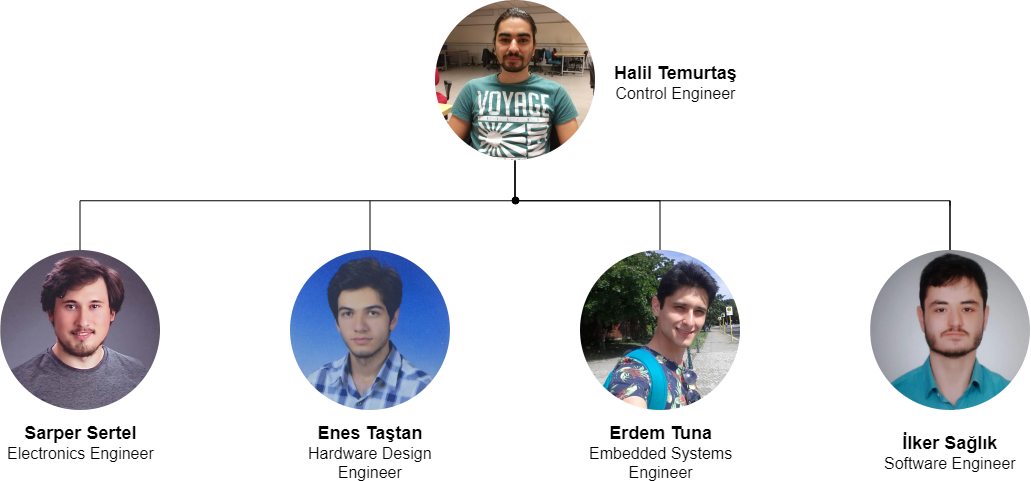
\includegraphics[width=\textwidth,height=\textheight,keepaspectratio]{../../Documents/company/company-tree} 
	\caption{\label{fig:company_tree}Company Tree of DUAYENLER.}
\end{figure}


\newpage

\section{Requirement Analysis}
	
	\subsection{Pairwise Comparisons for Project Selection}
		First, objectives of the project should be determined to select the project in a reasonable way. Pairwise comparisons technique can be used to assess the objectives of the project. Then, these objectives would be very useful in the assessment of the projects. As a result of the assessments, the desired project can be selected out of the rest. For this purpose, \textit{Table~\ref{tab:pairwise_comp}} and \textit{Table~\ref{tab:project_eval}} are created with the consensus of all company members. The weighted objectives are then used to construct the weighted objective tree in \textit{Figure~\ref{fig:objective_tree}}. 
		


	\begin{table}[H]
		\centering
		\caption{\label{tab:pairwise_comp}Pairwise Comparison Charts}\vspace{-.2cm}
		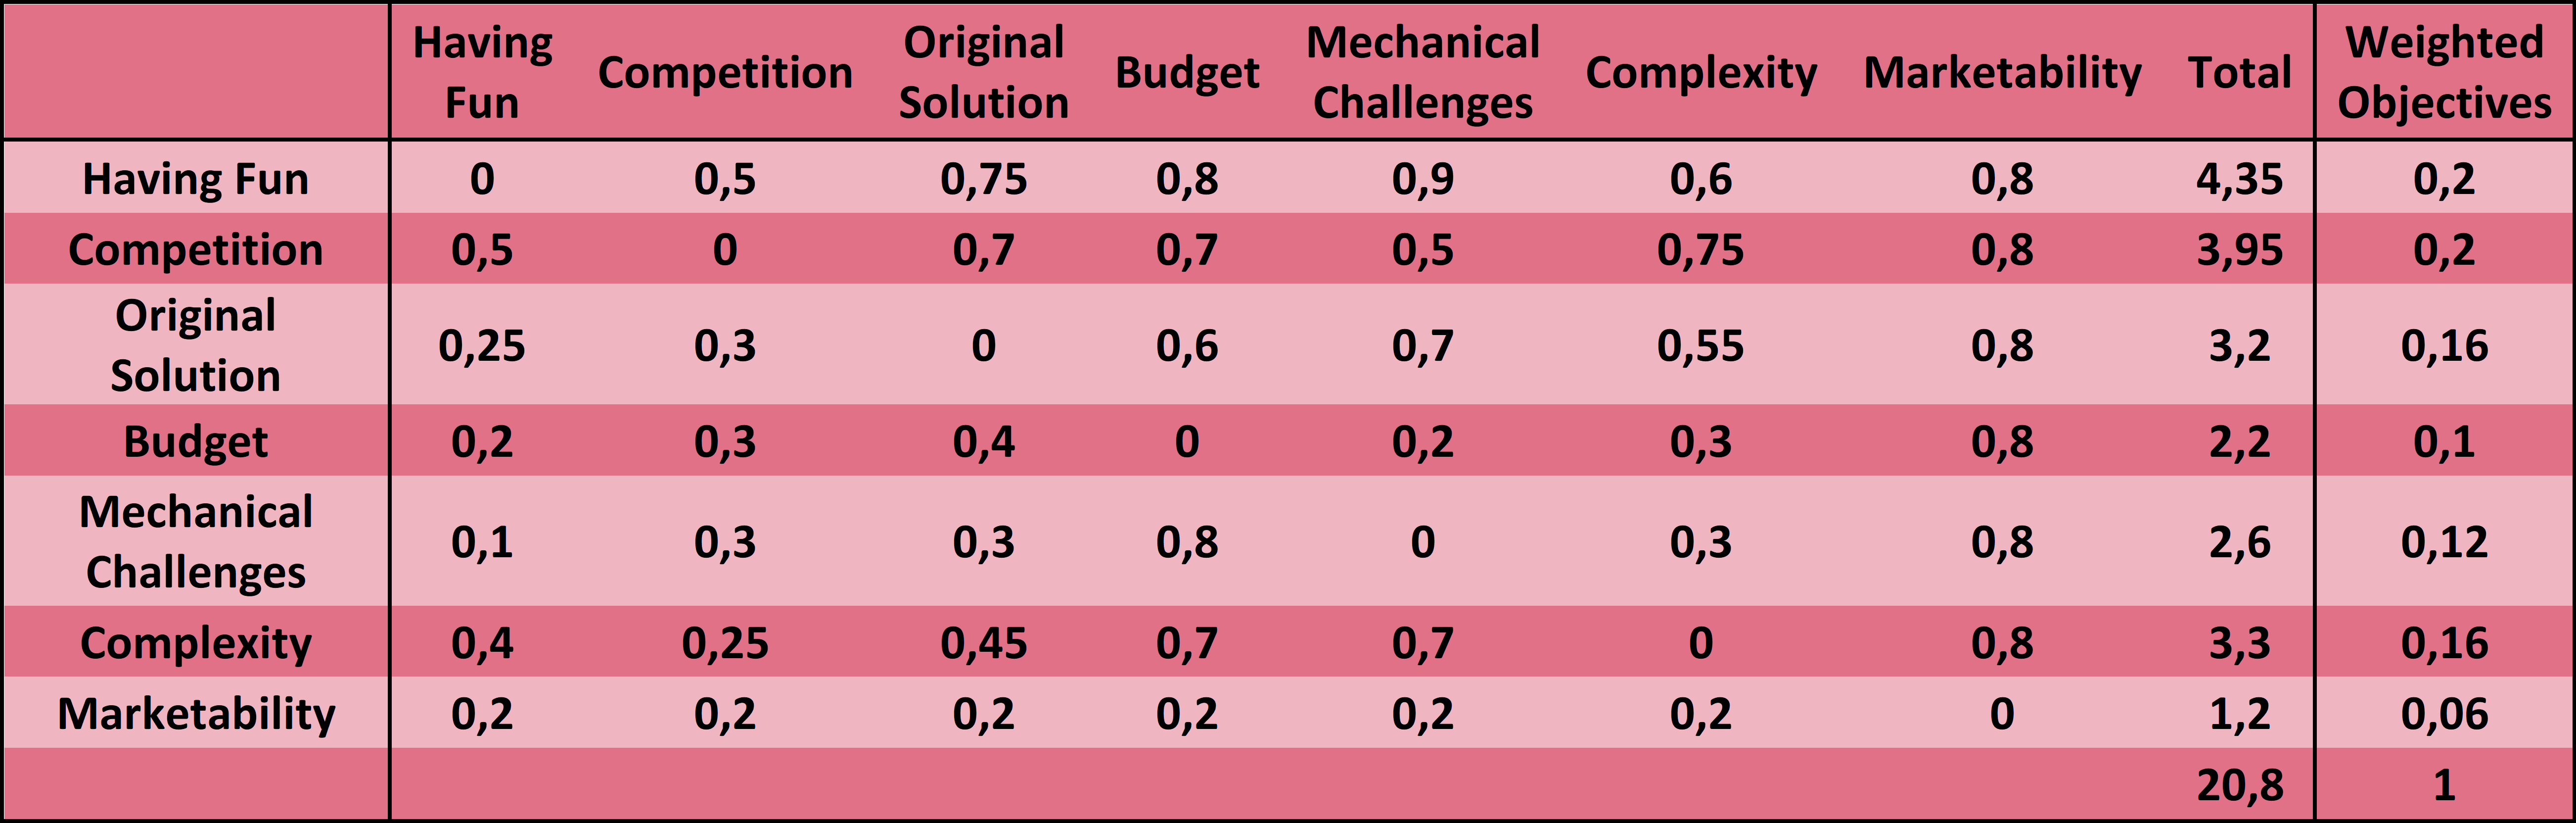
\includegraphics[width=\textwidth]{images/objective_tree3} 
	\vspace*{-.9cm}	\begin{center}
		{\small 0-0.2: No Importance, 0.2-0.4: Less Importance, 0.4-0.6: Equal Importance,\\ 0.6-0.8: More Importance, 0.8-1: Absolute Importance }	
		\end{center}
	\end{table}	\vspace*{-.5cm}	
	To determine the relative importances of objectives, the used method is as follows: If everyone is agreed on the importance value, that value is assigned as the comparison result. If there is a conflict between the members, the average of the proposed values are assigned as the importance of corresponding objective.
	\begin{figure}[H]
		\centering
		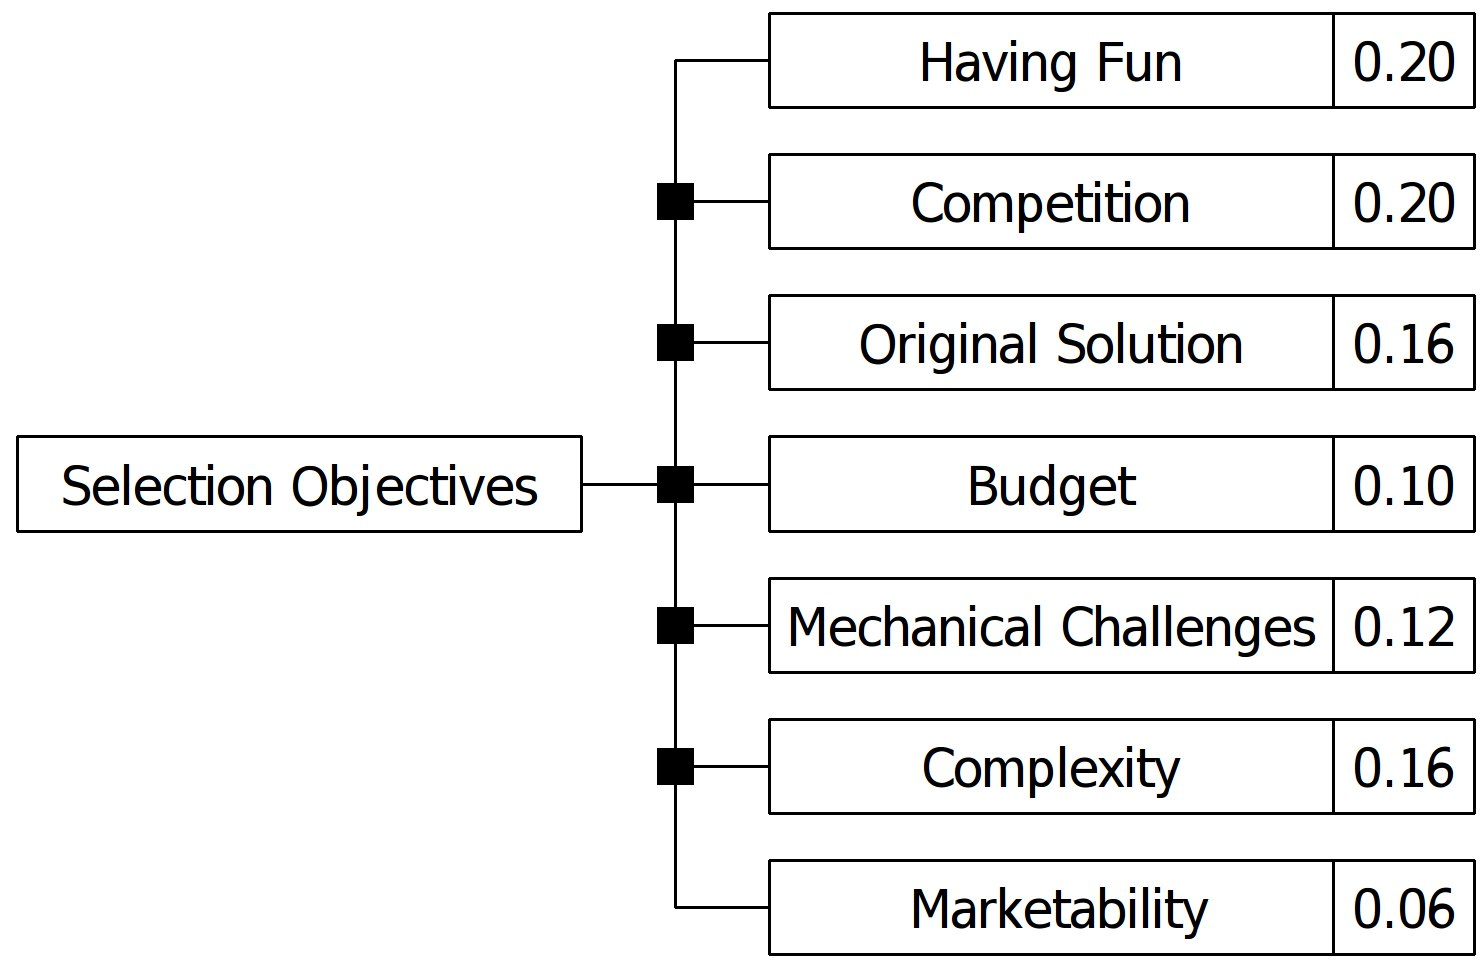
\includegraphics[width=.6\textwidth]{pre-objective-tree/pre-objective-tree} 
		\caption{\label{fig:objective_tree}Weighted Objective Tree}
	\end{figure}
	
	
	\subsection{Project Selection}	
	
		After selecting the objectives for the project, the possible projects were rated by the project members in a defined scale. The \textit{Table~\ref{tab:project_eval}} is constructed by using the same methodology as in the objective tree. The result of this chart is then used to choose which project will be developed. According to the \textit{Table~\ref{tab:project_eval}}, Chasing Car project is suited best for the objectives of the DUAYENLER. Thus, the Chasing Car project is chosen.
		
	\begin{table}[H]
		\centering
		\caption{\label{tab:project_eval}Project Evaluation Chart}\vspace{-.2cm}
		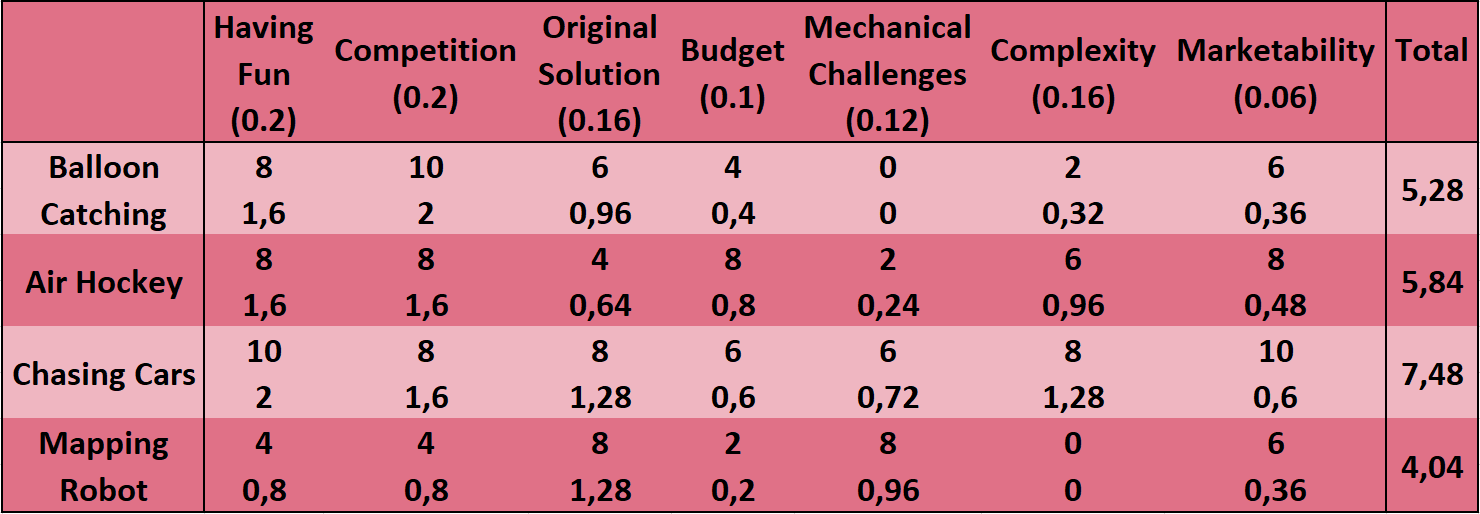
\includegraphics[width=\textwidth,height=\textheight,keepaspectratio]{images/project_evaluation4} 
	\vspace*{-.9cm}	\begin{center}
		{\small 0: Failure, 2: Unacceptable, 4: Average, 6: Satisfactory, 8: Good, 10: Excellent }	
		\end{center}
	\end{table}	\vspace*{-.5cm}	
	
	The aim of DUAYENLER is first to realize the project within the scope of the requirements. The foreseen mass manufactured cost of the project is limited to $\$$200. However, the research and development phase will cost up to 	$\$$450.
	
	\subsection{Statement of the Problem}
		
			The aim of the project is to design and construct a robot that can compete in a elliptic path with a similar robot in autonomous way.
			
			From this definition, it can be deduced that the robot should,
			\begin{itemize}
				\item detect start signal\vspace{-.2cm}
				\item detect path it is following\vspace{-.2cm}
				\item compute the curvature of the road\vspace{-.2cm}
				\item adjust wheels \& speed\vspace{-.2cm}
				\item catch the opponent\vspace{-.2cm}
				\item activate handshake protocol\vspace{-.2cm}
				\item stop\vspace{-.2cm}
			\end{itemize}
	
	
	\subsection{Pairwise Comparisons for Solution Selection}	
	
		In order to be able to compare the proposed solutions for the project, weighted objectives for the solutions should be formed to complete this task in a logical manner. The pairwise comparison chart for the solution objectives in \textit{Table~\ref{tab:sub_project_objective_tree}\ } is formed using same methodology that was used to construct the pairwise comparison chart for project objectives. Afterwards, the weighted objective tree at \textit{Figure~\ref{fig:product_tree}} is formed using the objectives selected.
	
	
	\begin{table}[H]
		\centering
		\caption{\label{tab:sub_project_objective_tree}Pairwise Comparison Charts for Sub-Objectives}\vspace{-.2cm}
		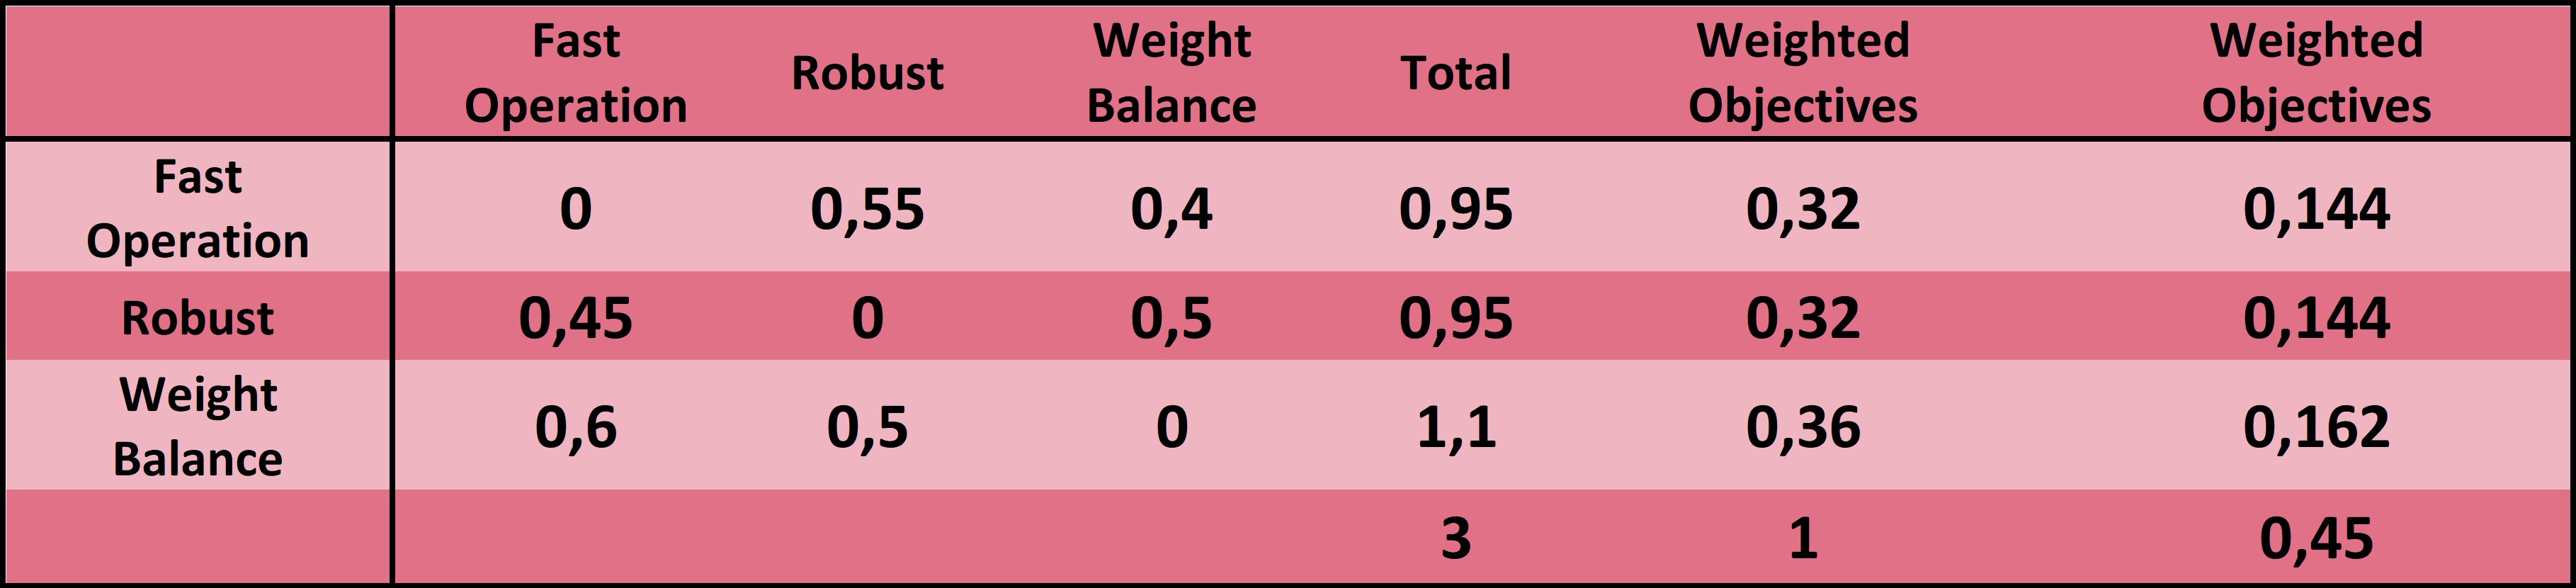
\includegraphics[width=\textwidth,height=\textheight,keepaspectratio]{images/proje_objective_tree_2a} 
	\vspace*{-.9cm}	\begin{center}
		{\small 0-0.2: No Importance, 0.2-0.4: Less Importance, 0.4-0.6: Equal Importance,\\ 0.6-0.8: More Importance, 0.8-1: Absolute Importance }	
		\end{center}
	\end{table}	\vspace*{-.5cm}
	
	\begin{figure}[H]
		\centering
		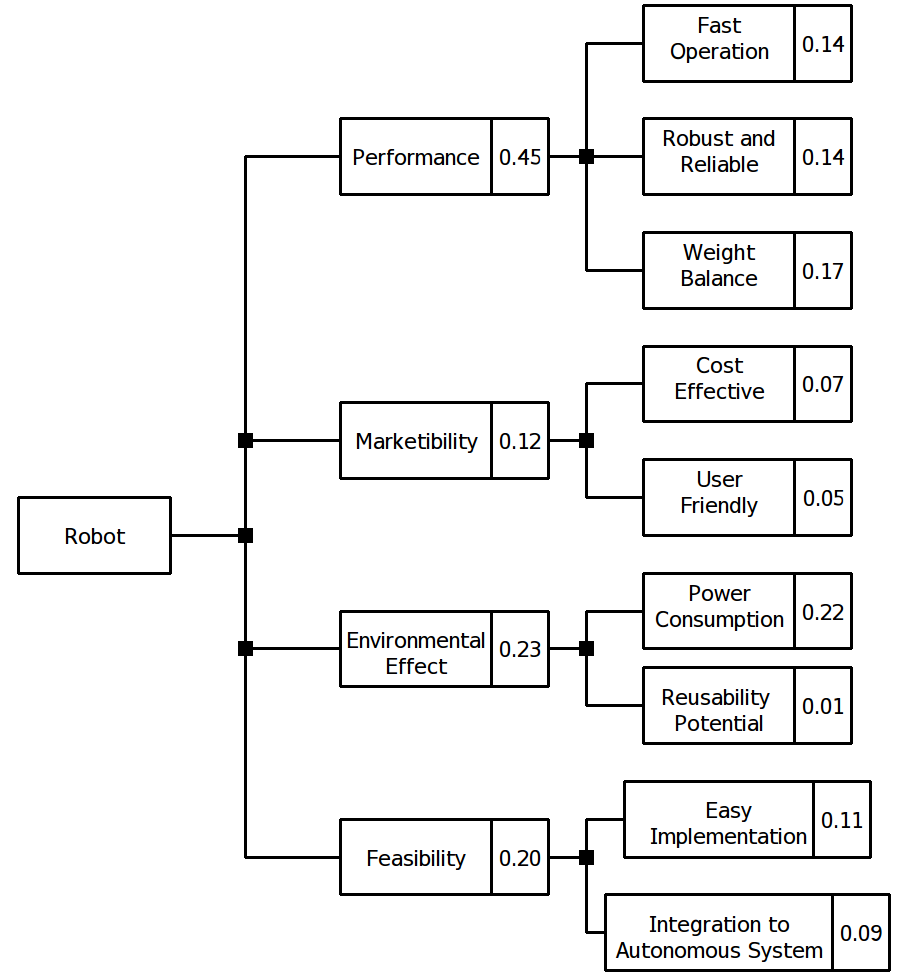
\includegraphics[width=.7\textwidth,center]{objective-tree/objective-tree} 
		\caption{\label{fig:product_tree}Weighted Objective Tree}
	\end{figure}
	
	
	
	\subsection{Systems \& Subsystems of Chosen Project}
		
	After choosing the project, the systems and subsystems of the project is determined by the group members. While disassembling the project to its systems, it is decided that the project will be investigated under two main parts, electrical and mechanical systems. Then, the electrical unit is then divided into three parts, that is, sensing, computation and driving subsystems. The mechanical system is also divided into two parts, that is, motion and structure subsystems. The system diagram of the chosen project can be seen at \textit{Figure~\ref{fig:system_diagram}}. System tree of the project can be seen at \textit{Figure~\ref{fig:systems_project}}.
	
	\begin{figure}[H]
		\centering
		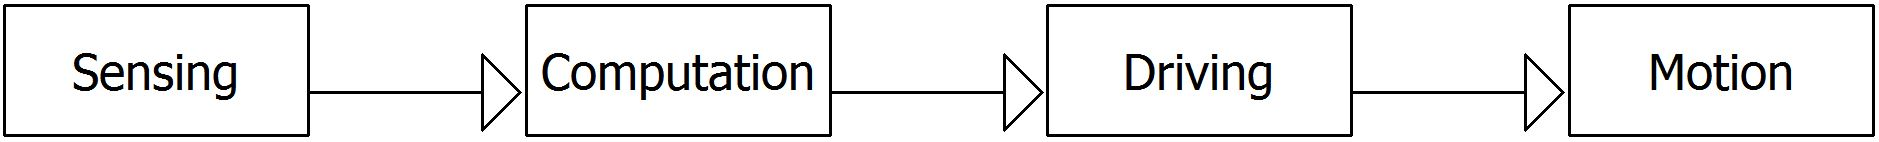
\includegraphics[width=\textwidth,height=\textheight,keepaspectratio]{product-tree/system-flow} 
		\caption{\label{fig:system_diagram}System Diagram for the Chosen Project}
	\end{figure}
	
	
	\begin{figure}[H]
		\centering
		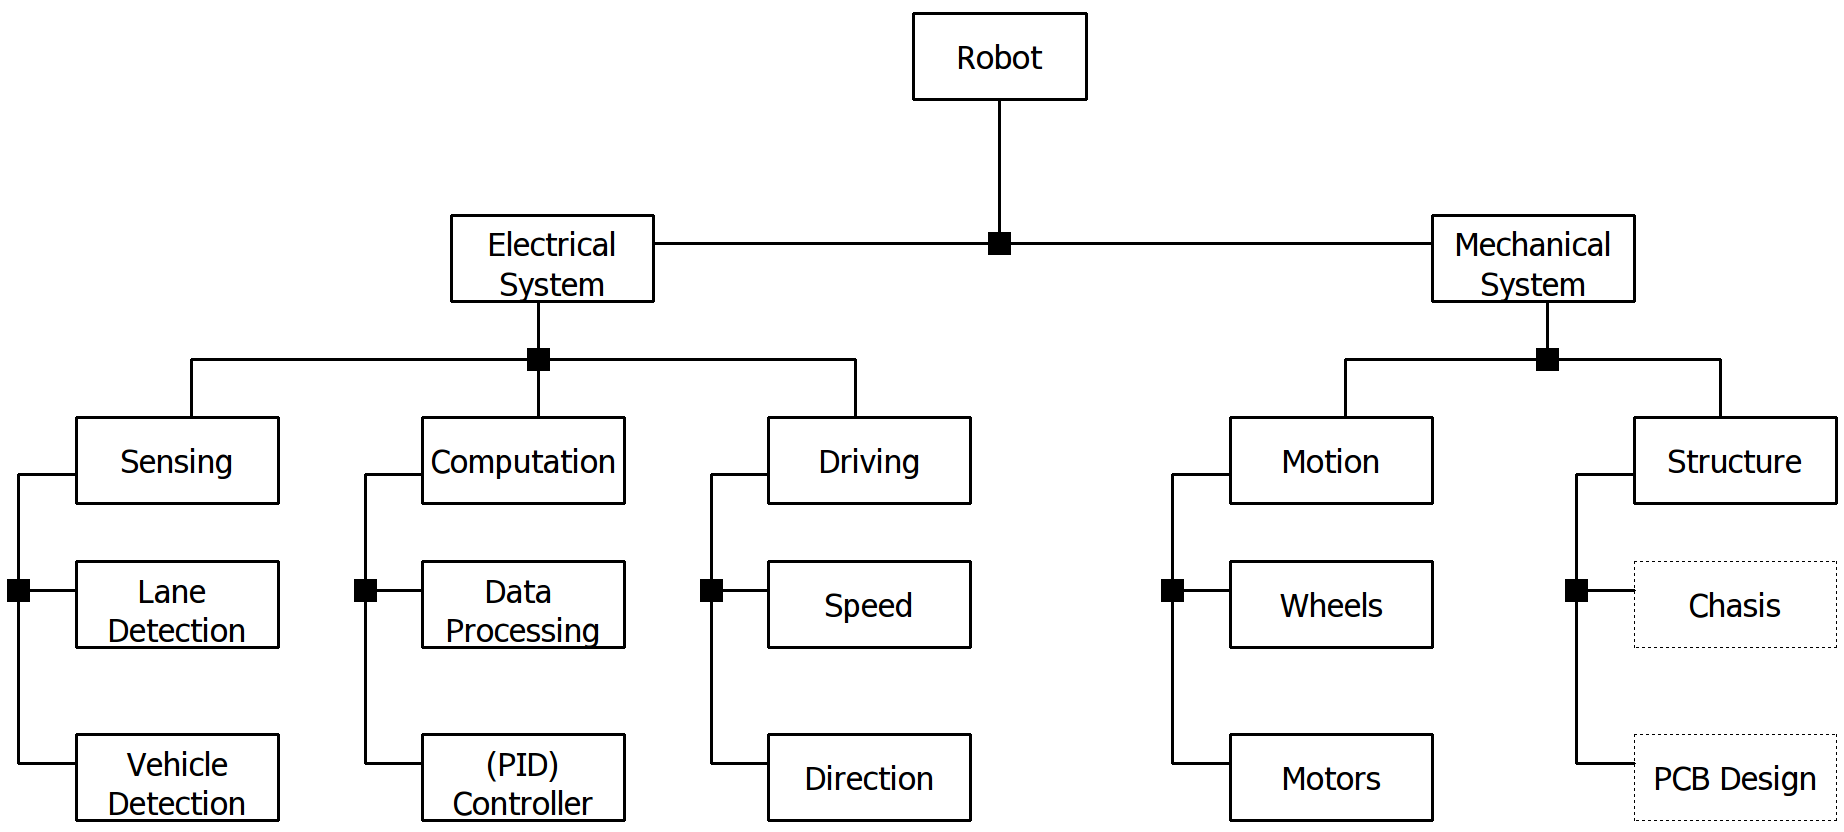
\includegraphics[width=\textwidth,height=\textheight,keepaspectratio]{product-tree/product-tree} 
		\caption{\label{fig:systems_project}Systems \& Subsystems of Chosen Project}
	\end{figure}

	\subsection{Solution Alternatives for Systems \& Subsystems }
	
	Following the division of the project into its sub-blocks, solution alternatives are created for these subsystems and units. 
		
	\begin{itemize}
		\item It is decided that the line detection unit will use sensor array to detect the borders of the path. The array might be consist of color sensors of infrared sensors. A camera might also be used to back up the sensor array for more reliable operation.	
		\item Vehicle detection unit might utilize ultrasonic, infrared distance sensors or camera in order to identify the opponent.
		\item  Arduino, Raspberry Pi or Asus Thinkerboard can be utilized as a microcontroller by the data processing unit.
		\item The controller unit can adopt P,PI or PID controller.
		\item Motor unit might consist of brushed or brushless motors.
		\item The project might consisist of three wheels (two of them are driven by DC motors and one of them is a ball caster), palette system(4+ Wheels) or four wheels (two of them driven by DC motors and two front wheels directed by servo motors)
		\item Speed unit might use only the output of the lane detection unit or the output data can be combined with gyroscope that can detect disturbances for speed reduction.  
		\item Direction unit might benefit from the advantages of differential drive or can combine these benefits with the servo motors that can determine the position of the front wheels.
	\end{itemize}	  
			
		The solution alternatives for units in compact form can be seen at \textit{Table~\ref{tab:solns}}.
	
\begin{table}[H]
  \centering
 	 \caption{Possible Solution Alternatives for the  Units of the Project}\vspace{-.2cm}
    \begin{tabular}{| c | c  c  c |}
    \hline 
    	&&& \\
       Unit & Possible Solution 1 & Possible Solution 2  & Possible Solution 3 \\ \hline
       &&& \\
       Lane Detection  & Color Sensor Array & Infrared Sensor Array & \specialcell{ Infrared Sensor  Array \\ with  Camera Support}  \\
       \hline 
       &&& \\
       Vehicle Detection & Laser sensor  & Ultrasonic sensor & \specialcell{Camera to back \\of the vehicle } \\

       \hline 
       &&& \\
       Data Processing & Raspberry Pi & Arduino & Asus Thinkerboard \\ 
       \hline 
       &&& \\
       Controller & P & PI & PID \\ 
       \hline 
       &&& \\
       Motors & Brushed Motors & Brushless Motors & \\
       \hline 
       &&& \\
%		Wheels & \specialcell{3 Wheels \\(2 Wheels with \\ DC Motors + \\ 1 Ball Caster) } &\specialcell{4 Wheels \\(2 Wheels with \\DC Motors + Palette)}  &\specialcell{4 Wheels \\(2 Wheels with DC Motors + \\2 Wheels with Servo Motors) }   \\
		Wheels & 3 Wheels  &  \specialcell{4 Wheels \\with Palette}  & \specialcell{4 Wheels \\with Servo Motors}   \\
		\hline 
		&&& \\
%		Speed & Lane Detection Output & \specialcell{Gyroscope (Balance Detection) \\to Speed Reduction}   \\
		Speed & \specialcell{Lane Detection \\Output} & \specialcell{Gyroscope \\(Balance Detection)}  & \\
		\hline 
		&&& \\
		Direction & Differential Drive & \specialcell{Servo Motors \\ for front wheels}   &
       
       
       \\\hline
      
  \end{tabular}
  \label{tab:solns}
\end{table}				
	
	
	\subsection{Design Options}
	
	After determining the possible solution alternatives, it is decided that these alternatives might be combined into design packages that can be compared with each other by using the selection objectives determined earlier.  In order the combine the solution ideas, three different design options according to their complexities are considered to ease the decision process. Named as design 1, most basic design is formed considering the simpler alternatives, design 2 is formed considering the more reasonable alternatives that would satisfy the expectations and the design 3 is formed considering the best possible outcome. The design alternatives in a comparable form can be seen at \textit{Table~\ref{tab:designs}}. 
	
	\begin{table}[H]
  \centering
 	\caption{Design Options for the Chosen Project}\vspace{-.2cm}
    \begin{tabular}{| c | c | c | c |}
    	\hline 
    	&&& \\
    	Unit & Design Option 1 & Design Option 2  & Design Option 3 \\ \hline
       Lane Detection  & Color Sensor Array & Infrared Sensor Array & \specialcell{ Infrared Sensor  Array \\ with  Camera Support}  \\ 
       & & & \\
       Vehicle Detection &   \specialcell{Camera to back \\of the vehicle }  & Ultrasonic sensor & Laser sensor   \\
       &&& \\ 
       Data Processing & Arduino & Arduino & \specialcell{Raspberry Pi+\\Arduino} \\ 
       &&& \\
       Controller & P & PI & PID \\ 
       &&&  \\
       Motors & Brushed Motors & Brushed Motors & Brushed Motors \\
       &&& \\
%		Wheels & \specialcell{3 Wheels \\(2 Wheels with \\ DC Motors + \\ 1 Ball Caster) } &\specialcell{4 Wheels \\(2 Wheels with \\DC Motors + Palette)}  &\specialcell{4 Wheels \\(2 Wheels with DC Motors + \\2 Wheels with Servo Motors) }   \\
		Wheels & 3 Wheels  &  \specialcell{4 Wheels \\with Palette}  & \specialcell{4 Wheels \\with Servo Motors}   \\
		&&& \\
%		Speed & Lane Detection Output & \specialcell{Gyroscope (Balance Detection) \\to Speed Reduction}   \\
		Speed & \specialcell{Lane Detection \\Output} &  \specialcell{Lane Detection \\Output} & \specialcell{Lane Detection \\Output +  Gyroscope }   \\
		&&&\\
		Direction & Differential Drive  & Differential Drive & \specialcell{Servo Motors \\ for front wheels}  
       
       
       \\\hline
      
  \end{tabular}
  \label{tab:designs}
\end{table}			
				

\subsection{Pairwise Comparisons for Design Selection}		
	
	The possible solution alternative at \textit{Table~\ref{tab:soln_selection}} are rated by using the weighted objective at \textit{Table~\ref{fig:product_tree}}. The methods used for project objectives is again used for pairwise comparison for the design selection.
	
	As expected, the total ratings for possible solutions is very similar since the aim of the DUAYENLER was not to select the exact solution procedure in this state but to choose where should be started. It is intended by the group to start from the Design 1 that is the most basic one and improving the design in performance wise to reach the Design 2 or 3 by conducting more tests on vehicle.	
		
	\begin{table}[H]
		\centering
		\caption{\label{tab:soln_selection}Pairwise Comparison Charts for Solution Selection}\vspace{-.2cm}
		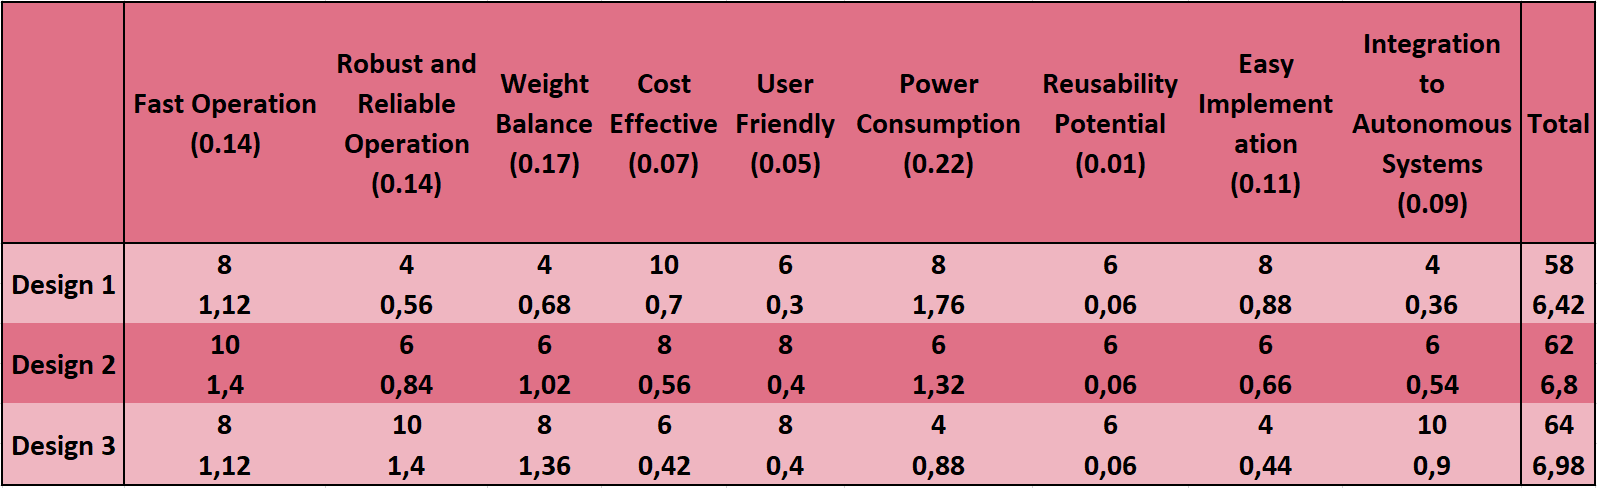
\includegraphics[width=\textwidth,center]{images/soln_selection3} 
	\vspace*{-.9cm}	\begin{center}
		{\small 0: Failure, 2: Unacceptable, 4: Average, 6: Satisfactory, 8: Good, 10: Excellent }	
		\end{center}
	\end{table}	\vspace*{-.5cm}	
	
	
\subsection{System Level Requirements}
	Under the light of the solutions, these system level requirements are constructed to achieve the customers needs.  
	\begin{itemize}
		\item The robot should follow the path in any circumstances
		\item The robot should complete the elliptical path in less than 15 seconds
		\item The robot should not crash the opponent
		\item The robot should function in any direction
		\item The robot should follow the handshake protocol decided by the committee
	\end{itemize}
	
	
	
	
	

%	\begin{figure}[H]
%		\centering
%		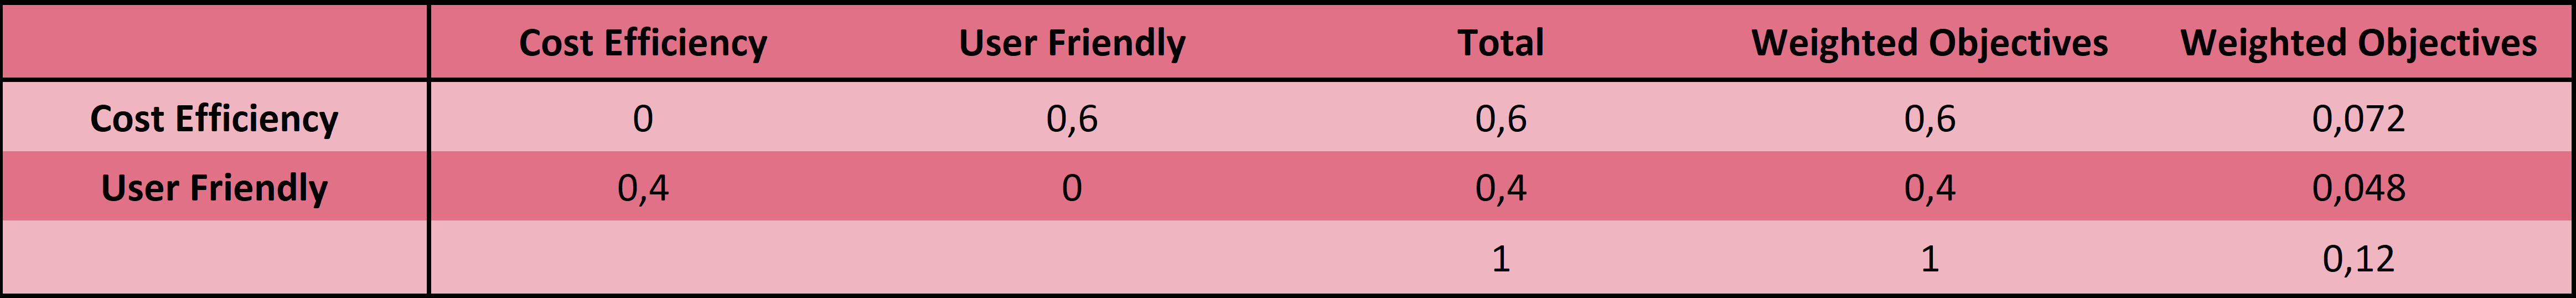
\includegraphics[width=\textwidth,height=\textheight,keepaspectratio]{images/proje_objective_tree_3} 
%		\caption{\label{fig:schedule}Weekly Schedule}
%	\end{figure}


%	\begin{figure}[H]
%		\centering
%		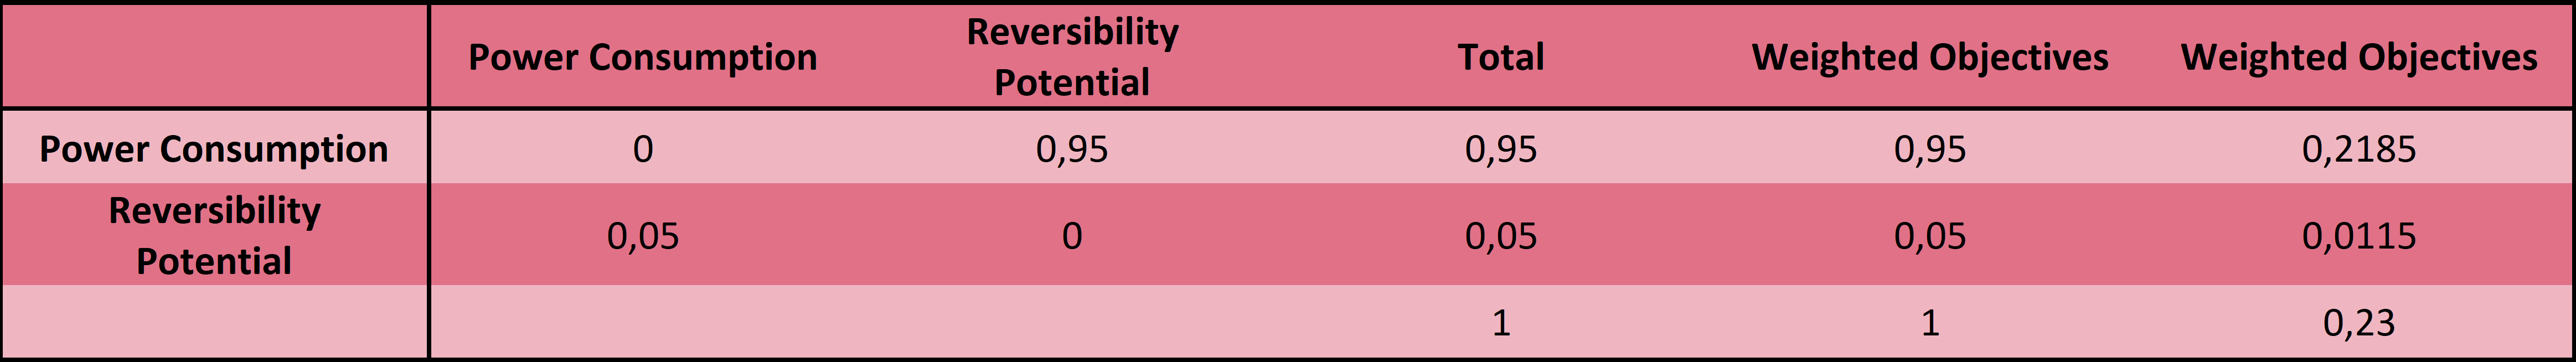
\includegraphics[width=\textwidth,height=\textheight,keepaspectratio]{images/proje_objective_tree_4} 
%		\caption{\label{fig:schedule}Weekly Schedule}
%	\end{figure}

	

\section{Standards Section}
Standards will be the base block that the project will be built on. There are several issues should be standardized before development phase. 

One of these issues is the handshake protocol. An option is using Bluetooth modules. When the distance between the two vehicles is less than 5 cm, both vehicles may send handshake signal to kill the motion. Benefit of this standard is that each vehicle needs to have only one distance sensor on the back or on the front. Another approach is having no communication protocol, but instead of this, each vehicle has 2 distance sensors which are placed back and front to detected each other, after detection, both vehicles stop individually. However, this method has a requirement that is detection platform. The reason obtain precise measurement. Otherwise, measurement may have error.  

Elevation of path is another problem that should be discussed. Some of the Infrared sensors operate between 0 to 15 mm, so after discussion, it can be decided whether or not use of the sensor. 

Braking criteria should be agreed by teams who chose this project because deceleration difference could cause collusion between the vehicle. Therefore, it should be standardized.      




\section{Solution Procedure}

\subsection{Milestones}
	Milestones are crucial steps to proceed in the development of the project. The steps of the project can be considered as successful, once the milestones are accomplished. The foreseen and planned milestones of the project are determined. The milestones are being able to,
	\begin{itemize}
		\item Move on a straight path  \vspace{-.2cm}
		\item Move on circular path \vspace{-.2cm}
		\item Move without crashing any object \vspace{-.2cm}
		\item Integrate camera vision to the vehicle  \vspace{-.2cm}
		\item Detect an elliptic path and moving on it \vspace{-.2cm}	
	\end{itemize}

	 
	
\subsection{Sensing Subsystem}
This unit has two main tasks which are observing lane and another vehicle on the path. 
\subsubsection{Lane Detection Unit}
To solve this problem, path and environmental differences, such as color difference, contrast difference could be used. In addition to these, image processing could be an alternative to detection of lane and vehicle. 
Infrared sensors can be used to solve lane detection problem. Line follower vehicle logic can be implemented to this problem, by placing two sensor arrays to both sides of the path to align vehicle at the center. Sensors gives current proportional to reflection of the surfaces. By using such outputs, an algorithm is to be developed to track the path on the center. 

Another approach to detect the lane is using camera and image processing. Camera can be placed at an angle to see the path, and by using the raspberry pi, the path can be followed. To clarify, captured frames can be analyzed by the raspberry pi, and utilizing open source image processing libraries. An example analysis can be summaries as follows: Firstly, distortions in the image can be beautified, and then color thresholding can be applied to sharply detect the elevated path. Optionally, to increase accuracy of the detection, Canny edge detection can be used. Lastly, center line can be calculated by using processed image. 

Color sensor can be utilized as an alternative for image processing. Color sensors basically senses the color with the help of 8x8 array of photodiodes and generates a PWM signal whose duty cycle is proportional to the light intensity. For example, if the elliptic path is red, we can give the s2 and s3 pins of the sensor low voltage, we activate the red photodiodes and we can use the Arduino command to measure the on or off time of the generated PWM signal. When the robots are out of the path, the output duty cycle of the sensor will significantly decrease, so this information can be used to keep the robots in the path. However, using color sensors can be problematic, because of their size and slow operation.

\subsubsection{Vehicle Detection Unit}
The detection of the opponent can be implemented using distance sensors. In order to stop the robot when it catches the opponent, or it is caught, a sensor must be placed at the front and the back. The most common distance sensors are ultrasonic, infrared and laser sensors. 

Ultrasonic sensors have acceptable range. They send a sound wave and take back the echo, then give a PWM voltage related to the distance. However, using ultrasonic sensors can cause problems if the opponent also uses ultrasonic sensors; because of the interference. Besides, when measurement is angled, measuring is failing. 

Infrared sensors can be another approach to this problem, they may provide better accuracy. Moreover, Laser distance measurement can be applied to solve this problem. They have the best accuracy, but their price is the highest among the rest.
\subsection{Computation Subsystem}
Functionality of computation subsystem will be presented in this section.
\subsubsection{Data Processing Unit}
This unit is the main algorithm application level. Data from sensor will be aggregated in this unit and will be pre-processed. Then, processed data will be output to the controller unit. Processing will mainly be done using Arduino and Raspberry Pi (if used). Suitable algorithms will be developed to realize desired operations with the controller unit

\subsubsection{Controller Unit}
Mathematical models will be implemented in this unit to realize controllers such as P, PI, PID. The output of the controller unit will be sent to driving subsystem. This output will be the ultimate decision to realize a desired operation according to the data sent from sensor.

\subsection{Driving Subsystem}
This unit takes an input from the controller unit. That input involves information about what the new orientation should be. Driving subsystem, then, takes action to move vehicle according to the required direction with maximum possible speed. This subsystem consists of two units: Direction and Speed.
\subsubsection{Direction Unit}
Direction unit is responsible for the orientation of the vehicle. It stores the last required orientation and the new one coming from the controller. After that, it tries to make the orientation as close as new one. Both data can be represented as vectors.The angle between those two vector is tried to be minimized by the controller. Before moving on to the operation, note that the angle can be used as a measure of the error that the direction unit have. The less the angle the more correctly operates the direction unit.\\

Depending on the configuration of the wheels, exact control of the vehicle might vary. However, there are certain methods to accomplish orientation. The vehicle will definitely have two wheels or palettes that will be driven by two separate DC motors. That configuration allows differential drive method to orient the vehicle. PWM values of the motors can be adjusted such that the speed difference between them results in a turn as much as desired angle. The exact difference values on the PWM values depends on the specs of the used motors and voltage sources. \\

Two different H-bridge motor drivers are proposed to be used to drive DC motors: L298N and L293D. Both can drive two motors separately with one IC. However, maximum current rating of the former one is larger being 2A while L293D can supply 0.6A per channel. \\

As in the case of another configuration that involves one or two servo motors to control the directions of the front wheels. This configuration is more robust compared to ball caster utilization. However, there are more motors to control and it requires more complicated differential drive algorithms involving both DC motor differential and servo PWM to orient the front wheels.
\subsubsection{Speed Unit}

This unit acts as a complementary module for direction unit. It will act as a state machine. In one state, the unit will try to increase the speed of the vehicle by making overall increase in both PWM values of DC motors. The feedback of this  system will be the cost function mentioned in driving unit. If that cost exceeds a specified level, unit goes to another state in which the unit will decrease the overall speed to allow direction unit to operate more correctly. In short, this unit tries to compensate the error of the direction unit by changing the overall speed of the vehicle.
 

\subsection{Structure Subsystem}
This part contains chassis and PCB sections of the robot. 
\subsubsection{Chassis Unit}
Main purposes of this section are protection of the critical elements of the robot and holding components together. The most important part of this section is weight distribution. The chassis is supposed to be light and strong because of the competition purposes. However, it should balance the robot to be able to handle with turns. 
\subsubsection{Printed Circuit Board Unit}
The main role of this part is decreasing connection mass and increase vibration strength of the robot against disturbances. Also, this section increases rigidity of the whole system. 
\subsection{Motion Subsystem}
Motion of the system is detailed in this section.
\subsubsection{Wheels Unit}
There are possible solution for wheel placement on the chassis, and several wheel types. Some wheels are designed for better gripping on different surfaces. To avoids obstacles on the path, gripping of the wheel is an important concept. Some wheel types are ball caster, toy car wheel and palette. Besides, wheel placement and the wheel number should be combined with the wheel type choice. 

One of the possible wheel placement is 2+1 combination. This combination can be assembled by placing 2 car wheels (with motors) to the back and the one boll caster to the front or vice versa. These configurations provide easy implementation and fairly reliable handling on the path. However, for certain obstacles may significantly disturb vehicles balance in this configuration.

Another combination is palette system. This system is used in real world where robust vehicles are needed. Similarly, this configuration can help handling obstacle in the path, but it costs for harder implementation and driving.

Last implementation is 2+2 configuration. In this configuration 2 wheels can be placed at the back and the rest at the front by placing motors to back wheels. To ease turning of the vehicle, front wheels can be controlled with a servo motor as back wheels operate in the differential drive mode. This combination may provide both enhanced grip and reliable	 operation. 
\subsubsection{Motors Unit}
Motors are one of the most important physical components of the project. There are possible motor types in the market.

One of the widely used motor type is brushed DC motors. Such motors might be implemented with gears. Gears are utilized to adjust torque and RPM of the motor, which is very suitable for a racing vehicle's needs. 

Another option is brushless DC motors. Brushless DC motors do not use brushes. This results in high torque. Brushless motors are more suitable for high RPM required areas such as CD drivers and drones.

Last option is servo motors. Servo motors are high-torque motors that can turn in an desired angle. Servos can be utilized in the direction of the vehicle on the front wheels. By using this solution, turning radius can be decrease significantly.

\section{Expected Deliverables}

The services and products that DUAYENLER Ltd. Şti. provides their customers can be listed as below.
\begin{itemize}
	\item A robot vehicle that is trying to catch the opponent in an elliptic path with varying width will be provided.
	\item The user will be provided with the elevated elliptical path with varying width.
	\item DUAYENLER Ltd. Şti. provides one(1) year warranty except the user faults.
	\item Also, a manual  which contains information about the usage of the vehicle will be included in the box. This manual will especially be helpful for the first usage of the device.
\end{itemize} 


\section{Conclusion}

\newpage
\begin{appendices}
	
		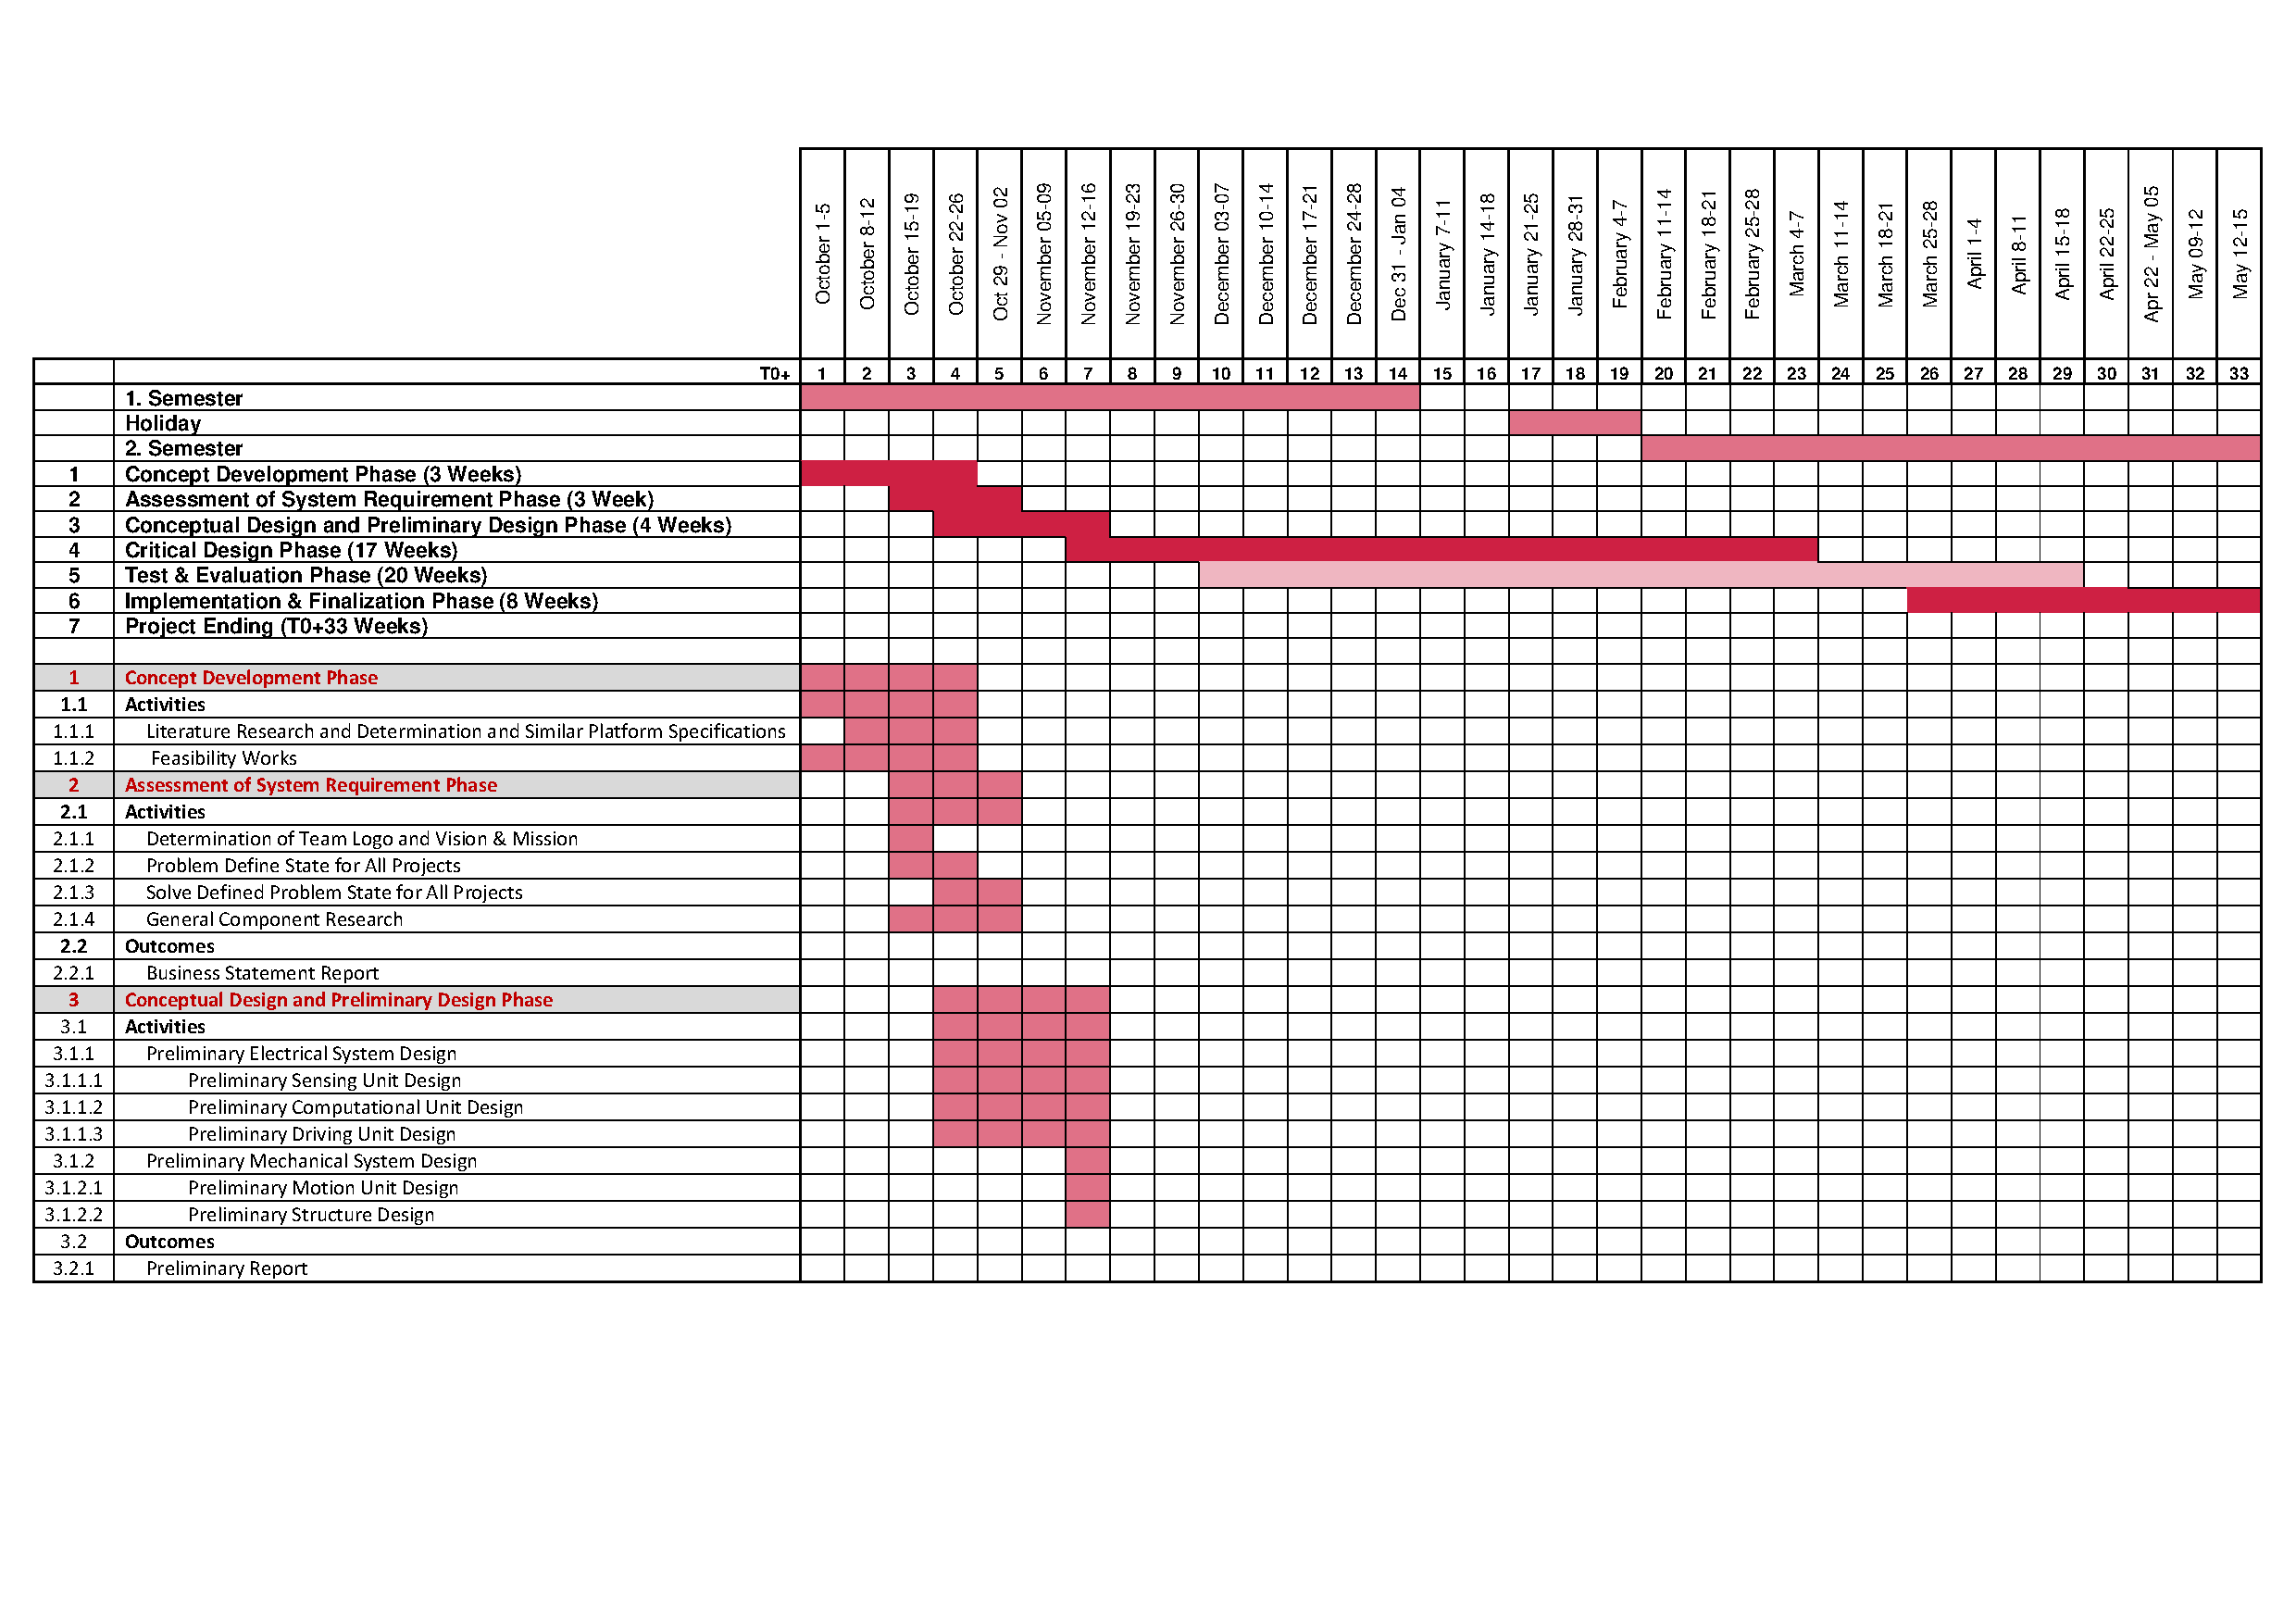
\includepdf[landscape=true,pages=1, scale=0.775,angle=0,pagecommand=\section{Gannt Chart}]{gannt2.pdf}
		\includepdf[landscape=true,pages=2, scale=0.775,angle=0,pagecommand=]{gannt2.pdf}

	
\end{appendices}




\end{document}

%----samples------
%\begin{itemize}
%\item Item
%\item Item
%\end{itemize}

%\begin{figure}[H]
%\center
%\setlength{\unitlength}{\textwidth} 
%
\includegraphics[width=0.7\unitlength]{images/logo1}
%\caption{\label{fig:logo}Logo }
%\end{figure}

%\begin{figure}[H]
%	\setlength{\unitlength}{\textwidth} 
%	\centering
%	\begin{subfigure}{.5\textwidth}
%  		\centering
%  		
\includegraphics[width=0.48\unitlength]{images/logo1}
%  		\caption{\label{fig:logo1}Logo1 }
%	\end{subfigure}%
%	\begin{subfigure}{.5\textwidth}
%  		\centering
%		
\includegraphics[width=0.48\unitlength]{images/logo2}
%  		\caption{\label{fig:logo2}Logo2}
%	\end{subfigure}
%\caption{\label{fig:calisandegree} Small Logos   }
%\end{figure}
	
%\begin{table}[H]
%  \centering
% 
%    \begin{tabular}{c|c|c}
%       $$A$$ & $$B$$ & $$C$$ \\ \hline
%       1 & 2 & 3  \\ \hline
%       2 & 3 & 4  \\ \hline
%       3 & 4 & 5  \\ \hline
%       4 & 5 & 6  
%      
%  \end{tabular}
%  \caption{table}
%  \label{tab:table}
%\end{table}
	
%\begin{table}[H]
%  \centering
% 
%    \begin{tabular}{c|c|c}
%       \backslashbox{$A$}{$a$} & $$\specialcell{ Average deviation \\ after subtracting out the  \\ frequency error }$$ & $$C$$ \\ \hline
%       \multirow{2}{*}{1} & 2 & 3  \\ \cline{2-3}
%        & 3 & 4  \\ \hline
%       3 & \multicolumn{2}{c}{4}  \\ \hline
%       4 & 5 & 6  
%      
%  \end{tabular}
%  \caption{table}
%  \label{tab:table}
%\end{table}
%-----end of samples-----